\subsection{Current implementation}
\label{sec:curr}

Currently, figshare holds all its metadata in a relational database \cite{figsupport}, with
tables for each of the entities required for describing a record. The reasoning behind
this choice includes the team's experience with relational systems, the extensive commercial
support for such solutions, and the high availability and clustering options provided by
these systems even before figshare's inception.

While the current system continues to function well, certain shortcomings were observed
when it came to implementing a number of features requested by figshare's users and customers; the two main requests that triggered the idea of using an RDF-based model are:

\begin{enumerate}
\item Provide the ability to export metadata in various formats, both predefined in the system and defined ad hoc by end users. Currently, figshare allows exporting metadata in a fixed set of
formats, both in its OAI-PMH interface and web application (see Fig. \ref{fig:figexport}), but this is
lacking in both number of formats and the actual metadata which is available when exporting (e.g., almost all options do not contain information about the files pertaining to a record).

\begin{figure}[thpb]
  \centering
  % fbox will add a border around the figure
  \fbox{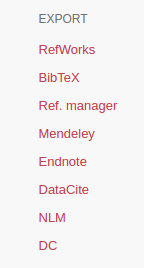
\includegraphics[scale=0.5]{figures/figshare_export.png}}
  \caption{Formats exposed by figshare for exporting bibliographical information via its web interface.}
  \label{fig:figexport}
\end{figure}

\item Provide an easy mechanism for enhancing the main metadata set. Currently figshare allows
institutional customers to define so-called \emph{custom metadata fields}, which extend the 
main set to include information such as, but not limited to, geographical
location information, retention dates, or archival markers; the interface for defining such fields
is presented in Fig. \ref{fig:caf}. The main limitation of these fields is that they currently
cannot be exported in any standard metadata format (e.g., via OAI-PMH) due to their lack of a
proper \emph{definition}; for example, when defining a field for holding geographical location
information, there is no mean of mentioning that this field follows the definition of the Dublin
Core Metadata Terms \emph{spatial} one (URI: \nolinkurl{http://dublincore.org/documents/dcmi-terms/#terms-spatial}). This limitation is not only one of the user interface, but also of the application's data model, as the relational scheme is not easy to modify in order to accommodate all the possible definitions and configurations.

\begin{figure}[thpb]
  \centering
  % fbox will add a border around the figure
  \fbox{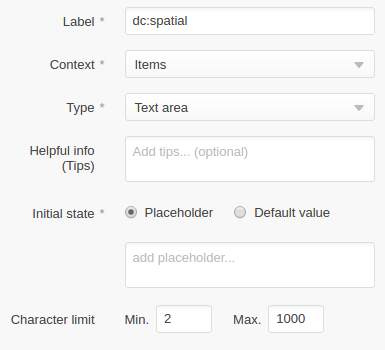
\includegraphics[scale=0.4]{figures/field.png}}
  \caption{Figshare interface that allows institutional clients to define custom metadata fields that can be filled in when creating a new record. Options for defining the type of the value (plain string, date field, etc.), certain validations, and guiding information are included.}
  \label{fig:caf}
\end{figure}

\end{enumerate}

While exploring possible solutions to the issues above it became clear that implementing an RDF-based model and workflows would be beneficial not only for answering the two requirements, but also for creating an extensible system upon which various use-cases can build upon. The solution is described in the next subsection.


\subsection{Towards an RDF model}
\label{sec:rdf}

The first challenge we need to overcome in building an RDF model is mapping all of figshare's metadata fields, defined as columns in the relational model, to a well-defined ontology, vocabulary of terms; this is required in order to
be able to properly identify the elements of the triples, as previously explained. In order to achieve this, we can either provide our own definition for each attribute in the relational model and then publish the whole set along with the RDF graph, or use an established vocabulary. We chose the second option, in order to comply with figshare's stated mission to use well-known standards, and avoid the \emph{not invented here} fallacy; moreover, this approach has already been explored by the figmeta project \cite{figmeta}, and this would speed up the development of our end-to-end solution.

Figmeta employs the VIVO Core Ontology \cite{vivo}. For each column in the relational model, the field in the ontology which is the closest to figshare's internal
\emph{definition} of the column's contents was chosen; it is worth noting that finding an objective measure of how well this mapping was done is quite difficult as figshare never provided an
exact meaning for each of the columns in the relational model (or metadata fields it expects its records to have). Having this ontology, triples describing a figshare item can be built,
and these can be visualized in a graph such as the one in Fig. \ref{fig:graph}.

\begin{figure*}[thpb]
  \centering
  % fbox will add a border around the figure
  \fbox{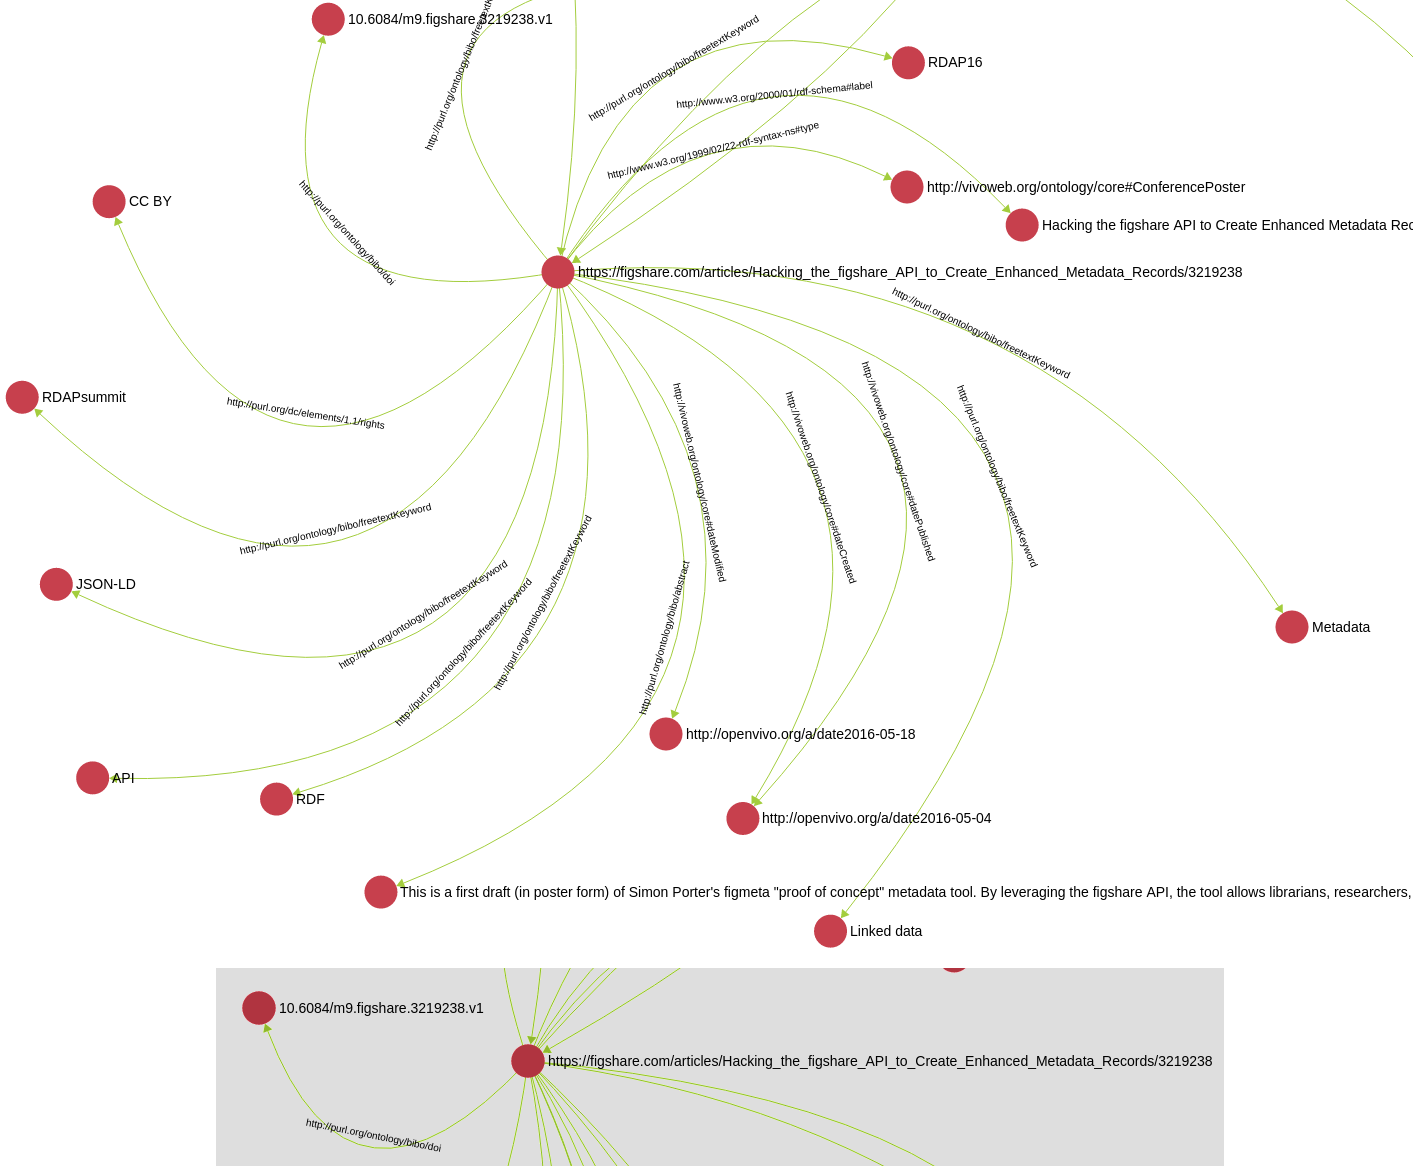
\includegraphics[scale=0.35]{figures/rdf.png}}
  \caption{A figshare item's RDF graph visualized. Vertices are subjects or objects, while edges are the predicates; edges are always directed from subject to object. The lower snapshot details one of the triples; the predicate is  from the BIBO ontology \cite{bibo}, used by VIVO, and associates the subject (a research record) with a Digital Object Identifier (DOI).}
  \label{fig:graph}
\end{figure*}

It is worth noting that this representation is already publicly available in the OAI-PMH interface, under
the RDF \emph{format}.

Our second challenge relates to the definition of custom, user-defined metadata. Here, we distance
from the approach taken by figmeta, which saved additional fields in a JSON-LD (a JavaScript Object Notation serialization of RDF triples) data file of the
record, by implementing an approach which embeds custom defined metadata in the original record
model. In order to achieve this, when defining a custom field, apart from the information
presented in Fig. \ref{fig:caf}, we also request the user to specify the ontology where the field
is defined (e.g., Dublin Core Metadata Terms), and its name in this ontology (e.g., \emph{spatial}).
This makes it very easy to include this new piece of information in the RDF graph; the predicate
becomes the term name and its ontology (e.g., \nolinkurl{http://dublincore.org/documents/dcmi-terms/#spatial}),
and the object the actual value, specified when the record is created. The subject, in the
current configuration, is always the figshare item, but due to the flexibility of the RDF model
it could become any other vertex in the graph (e.g., the file, or the author identifier).

Apart from the flexibility, this approach also has the advantage that it considers all metadata
to be equal. In the current relational model, where table structure cannot change so often, the
core metadata set, which was defined by figshare, is treated as a first-class citizen, while user
defined metadata is lacking certain features; for example, figshare's search system cannot fully search by the custom medatada fields (e.g., retrieve all records for which the \emph{spatial} field has the value ``Appalachian Mountains'', see the figshare search documentation at \cite{figsearch}). Our aim is to have a uniform representation, where all fields require equal effort in terms of development when a certain functionality is considered.

The third challenge we considered relates to the methods used for exporting metadata outside the figshare system. In the current model, this is done by implementing interfaces between the various aspects of the platform (OAI-PMH, web interface, RESTful API) and the relational model; this can become cumbersome, because for each new export format development time needs to be spent in order to provide it, and, even more important, users cannot define
their own preferred output.

RDF graphs can be serialized in various forms, such as the already mentioned JSON-LD, Turtle or N-Triples; the most popular one, nevertheless, is RDF/XML, which leverages the adoption of the XML format and its ecosystem. As most of the formats currently expected by figshare's users are
XML-based, we focused on this format, and noticed that starting from a RDF/XML serialization of our
graph we could easily pivot to any other format by employing Extensile Language Stylesheet Transformations (XSLT), a method for transforming XML documents to other XML representations.

Thus, for example, in order to get a Dublin Core Metadata Terms representation of a record modelled using RDF, two steps need to be performed:
\begin{enumerate}
\item Distil a RDF/XML serialization of the graph. Most RDF tools nowadays already include the means for this transformation, and thus, the development effort for this can be delegated to them.
\item Perform an XSL transformation from the RDF/XML document to the Dublin Core Metadata Terms one; in order to do this a stylesheet as the one in Fig. \ref{lst:xslt} can be employed. Tools for performing the actual transformation are also wide-spread.

\begin{figure*}[!ht]
\lstinputlisting[language=XML,
                 frame=tblr,
                 captionpos=b,
                 showspaces=false,
                 showstringspaces=false,
                 showtabs=false,
                 stepnumber=2,
                 numbersep=4pt,
                 basicstyle=\small]
  {figures/xslt.xml}
  \caption{Example XSL transformation for converting a RDF/XML document to Dublin Core Metadata Terms XML one.}
  \label{lst:xslt}
\end{figure*}
\end{enumerate}

An important advantage of this approach is that, starting from the XML/RDF serialization we provide, users can define their own transformations. This offloads the development work and
provides greater flexibility in terms of metadata output. The system also provides a solid
base for developing other internal features; for example, Fig. \ref{fig:tind_search} presents the way in which the Invenio digital library platform \cite{invenio} can output search results in the Metadata Object Description Schema (MODS) format; as this is also
an XML-based format, implementing the same functionality could be easily achieved via XSL transformations applied to RDF/XML.

\begin{figure*}[t]
  \centering
  % fbox will add a border around the figure
  \fbox{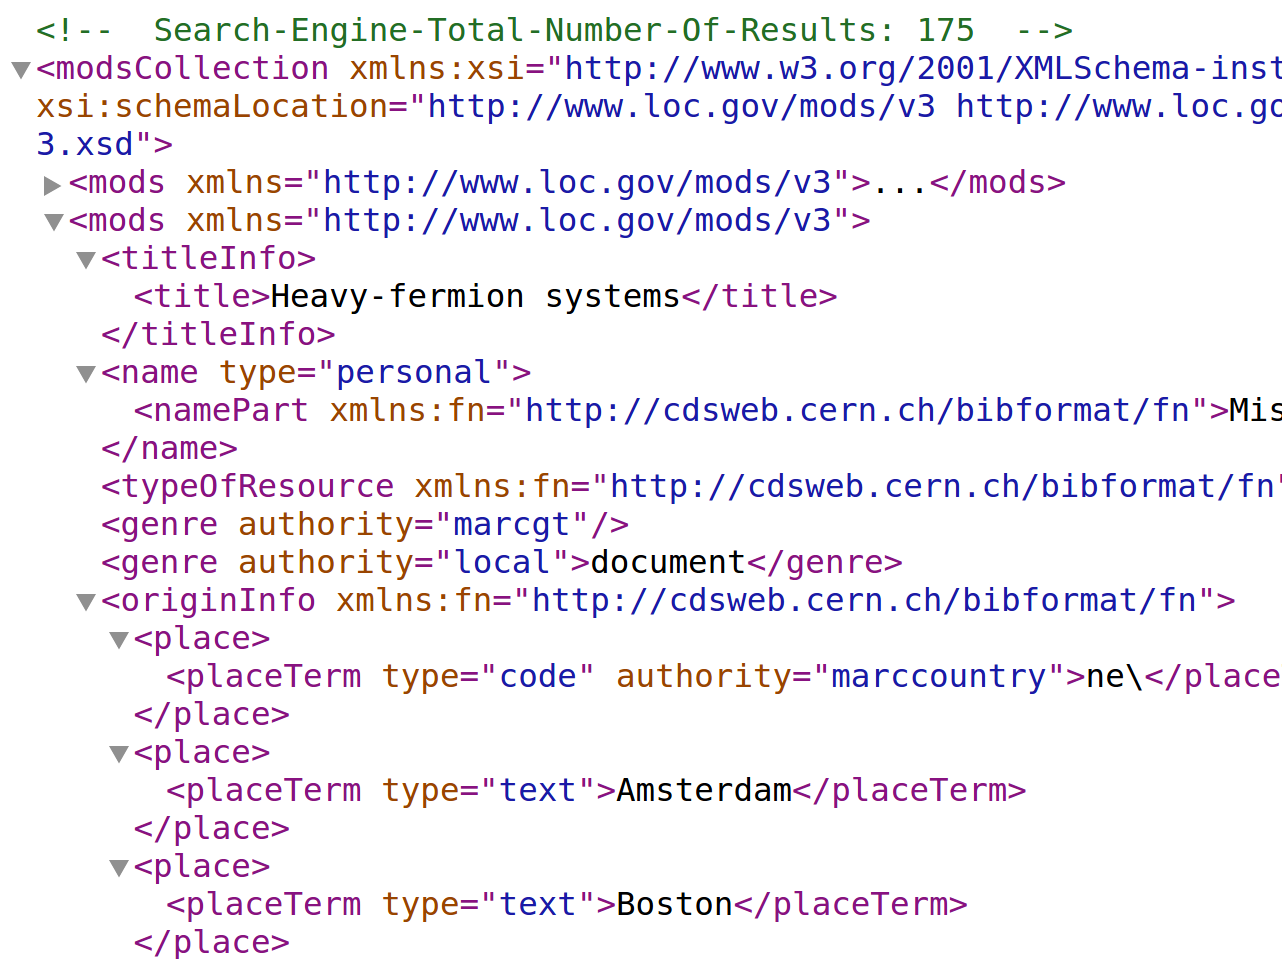
\includegraphics[scale=0.311]{figures/tind.png}}
  \caption{Search results in MODS format as returned by the California Institute of Technology Library Catalog \cite{caltech}, a solution using the Invenio framework.}
  \label{fig:tind_search}
\end{figure*}

Nevertheless, our system does not need to be limited to the RDF/XML representation; JSON-LD becomes more popular nowadays, especially because the predominance of the JSON format across web
applications, and RDF in Attributes (RDFa) starts being used by search engines for
achieving a better understanding of the indexed web pages \cite{googleld}.

%While a full implementation of the described system is not fully available, we provide a proof-of-concept one \cite{poc} which implements the uses-cases previously described and helped us understand the feasibility of the proposal and the ways in which we should proceed with the production-ready system. It is worth noting that for implementing the required operations we leveraged the RDFlib \cite{rdflib} and lxml \cite{lxml} Python libraries. 

After careful consideration, we reached the conclusion that completely replacing the relational model with the RDF one is not desirable, as, for example, we run the risk of loosing important business logic aspects. Instead, the two models can run in parallel, with the RDF one augmenting the current system. This, of course, will provide new challenges, such as maintaining the two sources of truth in sync while not limiting or hindering the operation of neither of them.